
%This is the hello world document, it is very usefull
%As you can see the character % is used for comments

\documentclass[a4paper,12pt]{article}
%\documentclass[doc]{apa}
\usepackage[usenames,dvipsnames]{color}
\usepackage{graphicx}
\usepackage{multicol}
\usepackage{multirow}
\usepackage{amsmath}
%\setlength\parindent{0pt}
%\usepackage{figure}
\usepackage[margin=0.8in]{geometry}
\title{Project 1. Content Based Image Retrieval Using Global and Local Features}
\author{Dan Bryan and Olmo Zavala}

\begin{document}
\maketitle

For this project three approaches for Content Based Image Retrieval  (CBIR)
where implemented. The first approach is based on the comparison of color 
histograms, the second solution uses spectral histogram to do the comparison,
of images and the third approach uses SIFT features to compare images. 

\section{Description}
In this section the three methods used for CBIR are described. 

\subsection{Color histogram}
\label{sec_colorhist}
In this method we used the color (intensity filter) histogram  to 
compare images. The following steps summarizes the method:
\begin{enumerate}
    \item \textbf{Image pyramidization. } The images sizes where reduced
        to half their size in order to speed up the algorithm. The method used
        to compute the pyramids is \emph{Gaussian pyramid}, the first
        step of the Gaussian pyramid algorithm is to blur the image 
        using a Gaussian filter, and then scale down the image by 
        creating one pixel from the average color of four pixels.
    \item \textbf{Compute histograms.} The number of bins used
        for this method is 256, for each color band.
    \item \textbf{Compute histogram distances.} The distance between
        each pair of image histograms were computed using histogram intersection:
        \begin{equation}
            dist(hist_a,hist_b) = \sum_{i=1}^{256} \min( hist_a(i), hist_b(i))
        \end{equation}
    \item \textbf{Images similarity}. The distance between the histograms
        of the images was used as the \emph{similarity} parameter. 
\end{enumerate}

\subsection{Spectral histogram}
\label{sec_spechist}
This method uses spectral histograms for CBIR. The proposed steps
for this method are the following:

\begin{enumerate}
    \item \textbf{Image pyramidization. } The images sizes where reduced
        to half their size in order to speed up the algorithm. The method used
        to compute the pyramids is \emph{Gaussian pyramid}, the first
        step of the Gaussian pyramid algorithm is to blur the image 
        using a Gaussian filter, and then scale down the image by 
        creating one pixel from the average color of four pixels.
    \item \textbf{Filter images}. Six filters plus the intensity
        filter are applied to each of the images. The filters 
        used and their corresponding masks are:
        \begin{equation}
            \begin{split}
                \frac{\partial I}{\partial x} & =  [0~-1~1] \\
                \frac{\partial I}{\partial y} & =  [0~-1~1]^T \\
                \frac{\partial I}{\partial x \partial x} & = [-1~2~-1] \\
                \frac{\partial I}{\partial y \partial y} & = [-1~2~-1]^T \\
                LoG(I(x,y))  & = ( x^2 + y^2 - \sqrt{2\sigma^2} ) e^{ -(x^2+y^2)/\sqrt{2\sigma^2}}\\
                Gauss(I(x,y))  & = \frac{1}{2 \pi \sigma^2} e^{ \frac{-(x.^2+y.^2)}{2\sigma^2}}\\
            \end{split}
        \end{equation}
        For the Laplacian of Gaussian (LoG) and Gaussian filters the size of the filter
        used is $5$ with a sigma value of $0.7$.
    \item \textbf{Compute spectral histograms.} The number of bins used
        for this method is 100, for each color band and for each filter. 
        For all the filters the range goes from [0 256], even when the values of some
        of the filters may go from [-256 256]. Several options for the range of the 
        histograms were tested, and the range of [0 256] gave the best results. 
        The 100 bins are evenly splitted from [0 256].
        Figure \ref{fig:spechist} shows an example of the spectral histograms. 
        \begin{figure}[h]
            \centering
            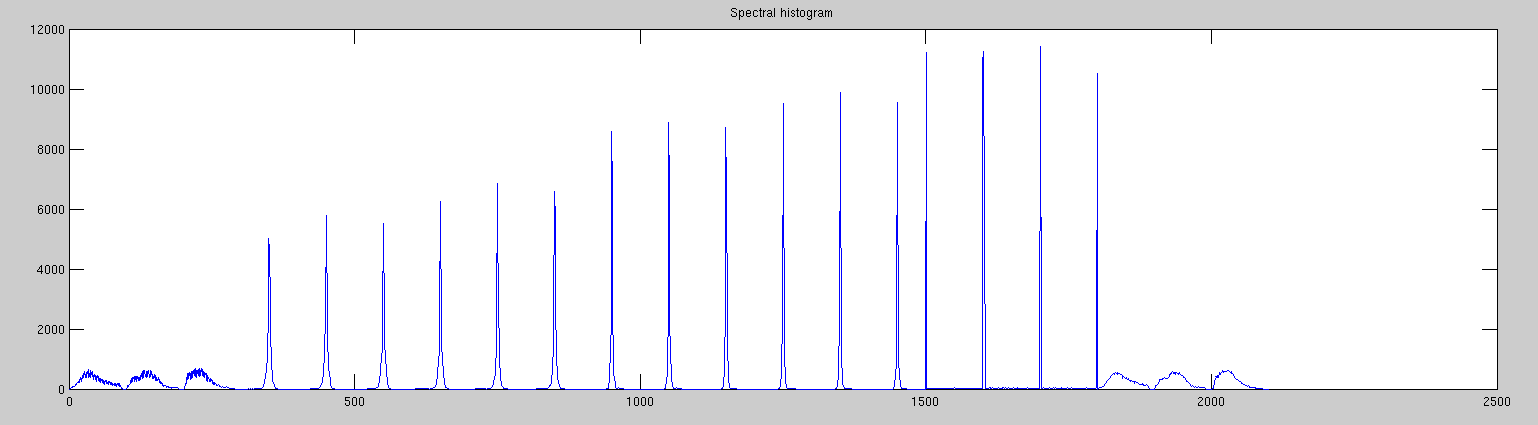
\includegraphics[totalheight=.18\textheight]{./Images/SpectralHist.png}
            \label{fig:spechist}
        \end{figure}
    \item \textbf{Compute histogram distances.} The distance between
        each pair of image histograms were computed using histogram intersection:
        \begin{equation}
            dist(hist_a,hist_b) = \sum_{i=1}^{100} \min( hist_a(i), hist_b(i))
        \end{equation}
    \item \textbf{Images similarity}. The distance between the histograms
        of the images was used as the \emph{similarity} parameter. 
\end{enumerate}

\subsection{Computation time}
The three methods were implemented in parallel (when possible) using the
matlab function $parfor$. The third method, which uses SIFT features,
takes a lot more time than the others and the computation time is presented separated
at the end of this section. \\

For eficiency, the first two methods are implemented in the same code, but the program 
\emph{Problem1And2CompTime} can be easily modified to display the time that
takes for each method to compute the CBIR. The times shown on table \ref{tab:times}
are for an specific run in a computer running Ubuntu 14.04, with matlab 2012a, 
with an i7 intel processor and 10 GB of ram. The times varies a little for each run
but table \ref{tab:times} gives a good estimate of the time that each method takes.
\begin{table}[h!]
    \centering
    \begin{tabular}{|c|c|c|}
        \hline
        & \textbf{Color histogram (sec)} & \textbf{Spectral Hist (sec)} \\
        \hline
        \textbf{Read Images} & & \\
        \textbf{Filter them and} & 9.38 & 30.01 \\
        \textbf{compute histogram} & & \\
        \hline
        \textbf{Compute distances} & 6.69 & 10.78  \\
        \hline
        \textbf{Compute Precision Recall } & 1.47 & 1.45 \\
        \hline
        \textbf{Avg Precision and Rank} & 1.22 & 1.34 \\
        \hline
        \textbf{Total time} & \textbf{17.54} & \textbf{43.58}\\
        \hline
    \end{tabular}
    \label{tab:times}
\end{table}

The method based on SIFT features take a lot longer to finish. In order to 
debug our proposed method, the computation of the SIFT descriptors were run once
and then saved in a separated file (\emph{/Variables/descriptors.mat}). In the same
way the matching of the descriptors, which takes almost two hours to finish,
was also saved in a separated file (\emph{/Variables/scores.mat}). In this way
we only had two compute the matching and the descriptors one time. 

\begin{table}[h!]
    \centering
    \begin{tabular}{|c|c|}
        \hline
        & SIFT (time sec) \\
        \hline
        \textbf{Read all Images} & 12.47 \\
        \hline
        \textbf{Detect SIFT descriptors} & 83.3 \\
        \hline
        \textbf{Matching descriptors} & approx. 7 sec/image\\
        & $\sim$ 7000 sec $\sim$ 1:56 hrs\\
        \hline
        \textbf{SIFT score} & 18.8 \\
        \hline
        \textbf{Precision recall} & 1.6 \\
        \hline
        \textbf{Average PR} & 1.44 \\
        \hline
        \textbf{Total} & $\sim$ \textbf{2 hrs}\\
        \hline
    \end{tabular}
    \label{tab:sift}
\end{table}

\section{Results}

To better display the results obtained with each method, the
results are plotted in one figure. 

One good image 401
\begin{figure}[h!]
    \centering
    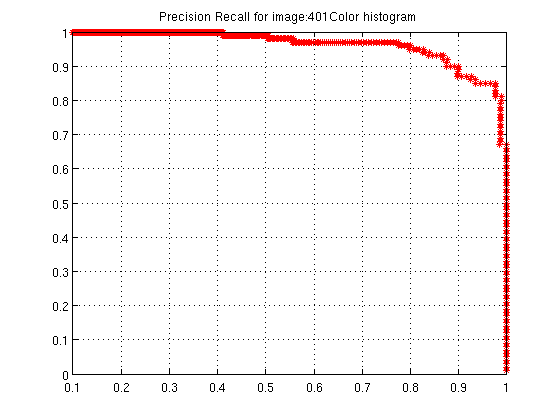
\includegraphics[totalheight=.24\textheight]{../Results/PR/GoodColor.png}
    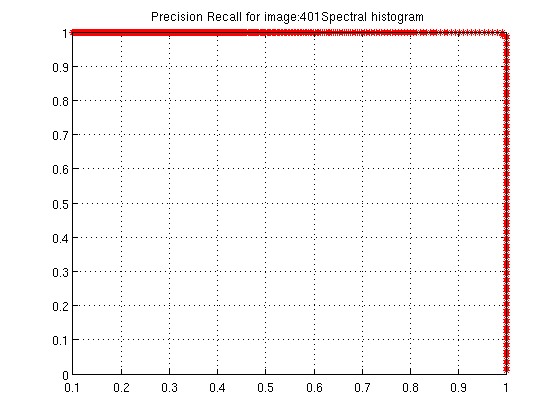
\includegraphics[totalheight=.24\textheight]{../Results/PR/GoodSpectral.png}
\end{figure}

One bad image 1
\begin{figure}[h!]
    \centering
    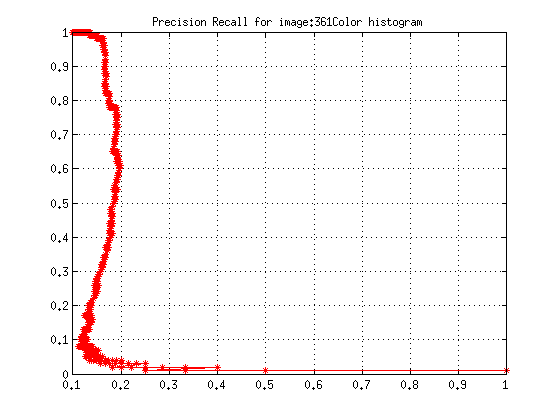
\includegraphics[totalheight=.24\textheight]{../Results/PR/BadColor.png}
    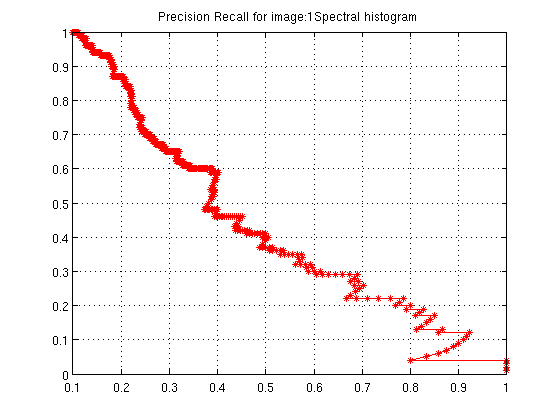
\includegraphics[totalheight=.24\textheight]{../Results/PR/BadSpectral.png}
\end{figure}



\end{document}
